\documentclass[12pt, a4paper, oneside]{ctexart}
\usepackage{amsmath, amsthm, amssymb, graphicx, fancyhdr}
\pagestyle{fancy}
\title{非甾体抗炎药的合理使用与开发}
\author{生信 2001 张子栋\thanks{E-mail: zidongzh@outlook.com}}
% 去掉日期
\date{}
% 页眉
\lhead{华中农业大学}
\rhead{药物化学结课论文}

% 正文部分
\begin{document}

\maketitle
\thispagestyle{empty}
\newpage

\tableofcontents

\thispagestyle{empty}
\setcounter{page}{0}

\newpage

% 摘要部分
\begin{abstract}
    非甾体抗炎药是生活中较为常用、适应症多的一种药物,
    通常用于消炎、止疼(如布洛芬缓释胶囊)和退热(如扑热息痛(对乙酰氨基酚))。
    另外在施用剂量较大时也有抗血栓作用。
    此类药物的副作用也十分明显,因此不宜长期服用或同类药物联用。
    目前此类药物已经十分成熟,新药研制方面也有许多不同的方向。
\end{abstract}

\textbf{关键字:}非甾体抗炎药、止疼、炎症、环氧化酶

\newpage
\section{非甾体抗炎药的定义}
\subsection{非甾体抗炎药的分类}
非甾体抗炎药可以通过多种方法分类。
由于其直接作用于环氧化酶,可以通过是否特异性作用于环氧化酶 II 
将其分为非选择性非甾体抗炎药和选择性非甾体抗炎药。
从化学本质上分类,可分为多氨基酚类、水杨酸类、烯醇酸类、乙酸类、吡唑酮类、昔布类。

\subsection{非甾体抗炎药的性质}
\subsubsection{甾体与非甾体抗炎药}
甾(z\=ai)体也译作类固醇 (steroid) 或糖皮质激素。译作这个生僻字「甾」并不是中国科学家故作高深,
建起学术壁垒,反而体现了汉字作为象形字的魅力,「巛」代表了侧链,「田」代表了四个环\cite{ref1}。
如下图 1\footnote{Guillem d'Occam - CC BY-SA 3.0},胆固醇也是一种甾体。

\begin{figure}[htbp]
    \centering
    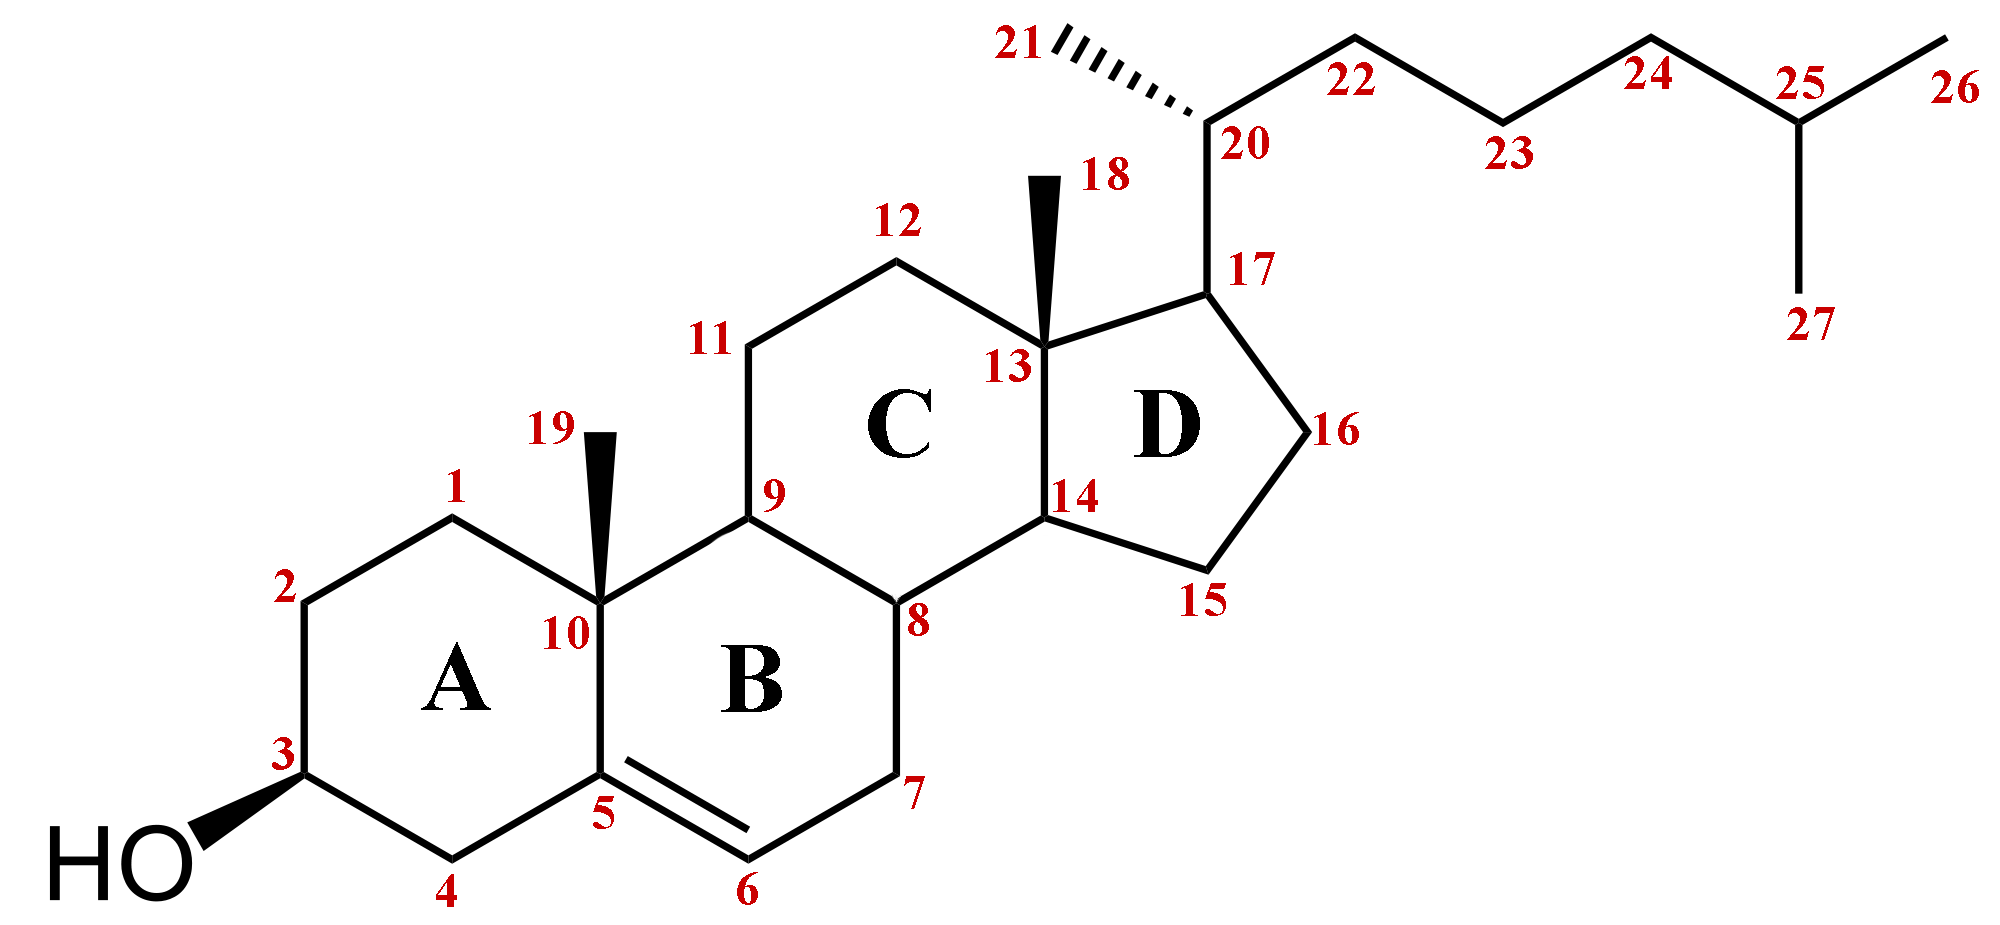
\includegraphics[width=10cm,height=4.625cm]{Colesterol.png}
    \caption{胆固醇 Colesterol}
\end{figure} 

甾体在生物体内主要作为激素,甾体类药物具有很强的消炎和免疫抑制作用,但同时也具有很大的副作用。
2003 年在我国爆发的非典疫情中,由于缺乏抗病毒药物,多数重症患者均使用了糖皮质激素进行治疗,
并且治疗效果良好。但在使用糖皮质激素治疗的患者中,均不同程度的出现了股骨头坏死的后遗症,
据研究股骨头坏死与使用大量糖皮质激素有一定关系\cite{ref2}。

由于甾体类药物的副作用较大,新的具有抗炎作用的非甾体药物被研制出来。为了与具有抗炎作用的甾体区分开,
这类药物取名非甾体抗炎药 (Non-Steroidal Anti-Inflammatory Drugs, NSAIDs)。
1952 年保泰松,并开始使用 NSAIDs 这个名称。

\subsection{非甾体抗炎药的历史沿革}
非甾体抗炎药这个名称是在 1952 年开始使用,但是第一种非甾体抗炎药问世的时间要早得多。
很久以前,人们就发现柳树皮具有一定的抗炎退热作用,并在 1838 年成功从柳树皮中提取出水杨酸,
在 1860 年实现了水杨酸的人工合成。之后在 1899 年拜尔公司将水杨酸的酚羟基乙酰化
(如图 2\footnote{By File:Aspirin-skeletal.svg originally by Benjah-bmm27 and Booyabazooka, edited by Fvasconcellos - File:Aspirin-skeletal.svg, Public Domain}),
推出阿司匹林,并迅速成为世界上使用最广泛的药物之一。

\begin{figure}[htbp]
    \centering
    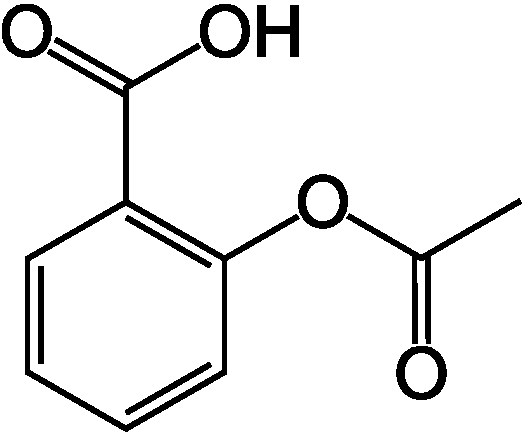
\includegraphics[width=4cm]{Aspirin-skeletal.pdf}
    \caption{阿司匹林 Aspirin}
\end{figure}

之后还出现了对抗疟药物奎宁进行改造的吡唑酮类药物,但由于其可能引起白细胞减少、粒细胞缺乏
的不良反应,已经被淘汰。目前市面上被广泛使用的主要为布洛芬这一类的芳基烷酸类非甾体抗炎药。

\newpage
\section{非甾体抗炎药的作用及其作用原理}
\subsection{非甾体抗炎药的作用}

非甾体抗炎药的主要作用是镇痛抗炎,另外还有退热和抗血栓的作用。
因为其抑制了会导致炎症和疼痛的前列腺素 (Prostaglandin, PG) 的合成,
另外在下丘脑中前列腺素还有调节体温的效果,所以对前列腺素的抑制能起到镇痛、消炎和退热的效果。
同时非甾体类抗炎药还能抑制具有凝集血小板作用的血栓素。

以上几种作用基本是所有非甾体抗炎药的共同特点,每种不同的非甾体抗炎药还有一些其他的效果。

\subsection{前列腺素与血栓素的作用}
\subsubsection*{前列腺素}
前列腺素从化学本质上来说是一类具有五元环和两个侧链的酸,是人体内的一种激素。
由于最初在前列腺液中被发现,故称前列腺素,具有收缩血管和平滑肌的作用,在体内其他地方也有分布。

\begin{figure}[htbp]
    \centering
    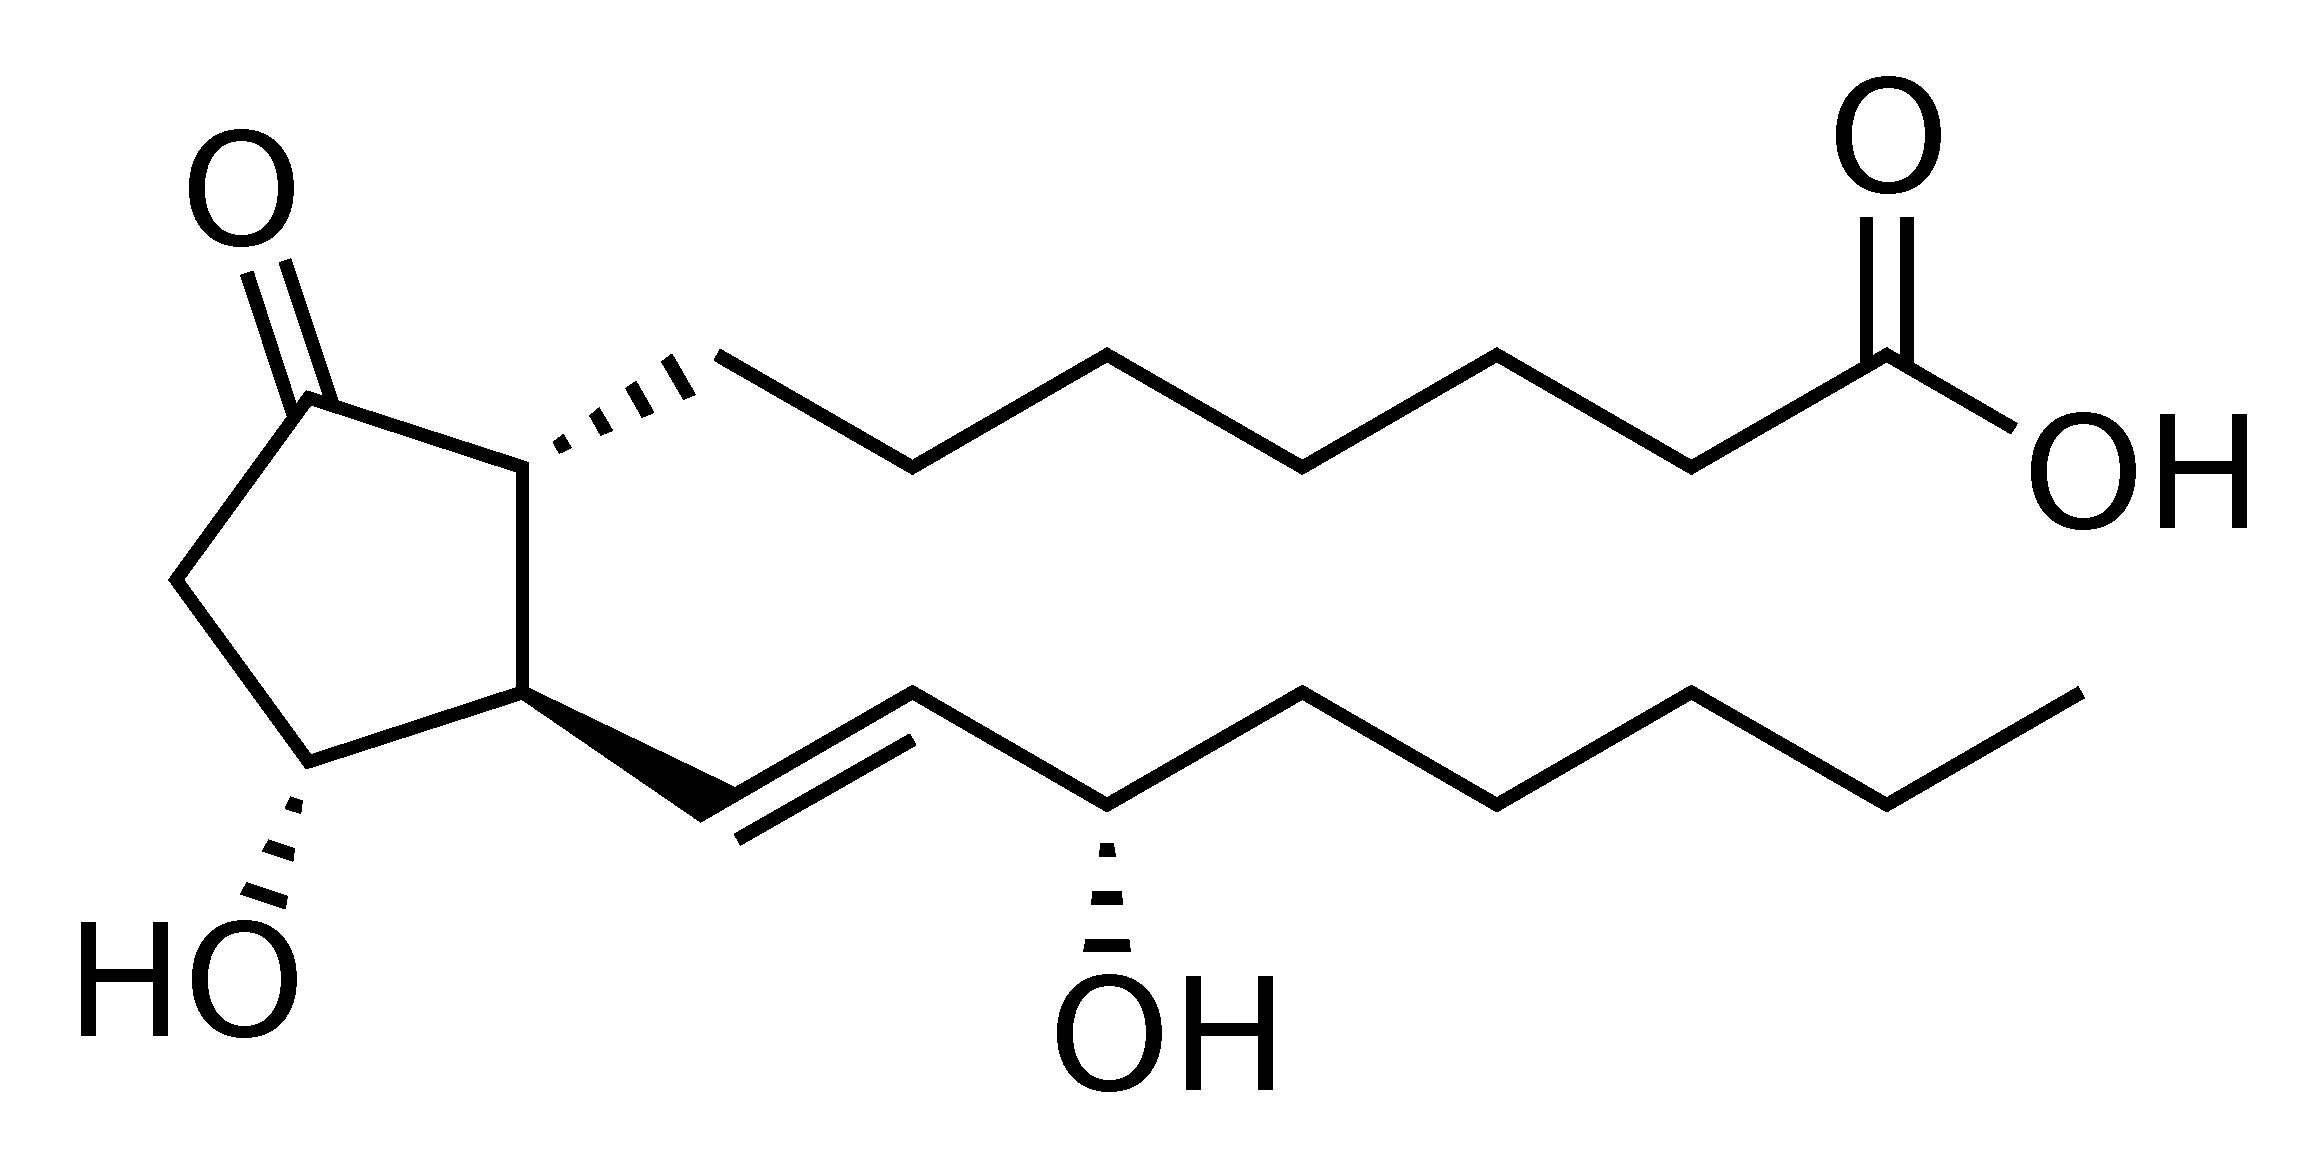
\includegraphics[width=6cm]{Prostaglandin_E1.pdf}
    \caption{前列腺素 $\mathrm{PGE_1}$}
\end{figure} 
\footnotetext[3]{Calvero. - Selfmade with ChemDraw.}

前列腺素的前体是花生四烯酸,前列腺素是一种炎症因子,会引起炎症。
另外 $\mathrm{PGE_1}$ 或 $\mathrm{PGE_2}$ 和 $\mathrm{PGA}$ 能抑制胃酸分泌,具有保护胃黏膜的作用。

\newpage

\subsubsection*{血栓素}

\begin{figure}[htbp]
    \centering
    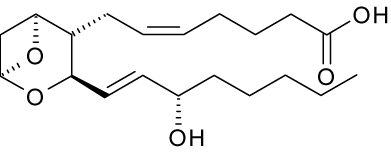
\includegraphics[width=6cm]{Thromboxane_A2.png}
    \caption{血栓素 $\mathrm{A_2}$}
\end{figure} 
\footnotetext[4]{Wikipedia. - CC BY-SA 3.0}

\begin{figure}[htbp]
    \centering
    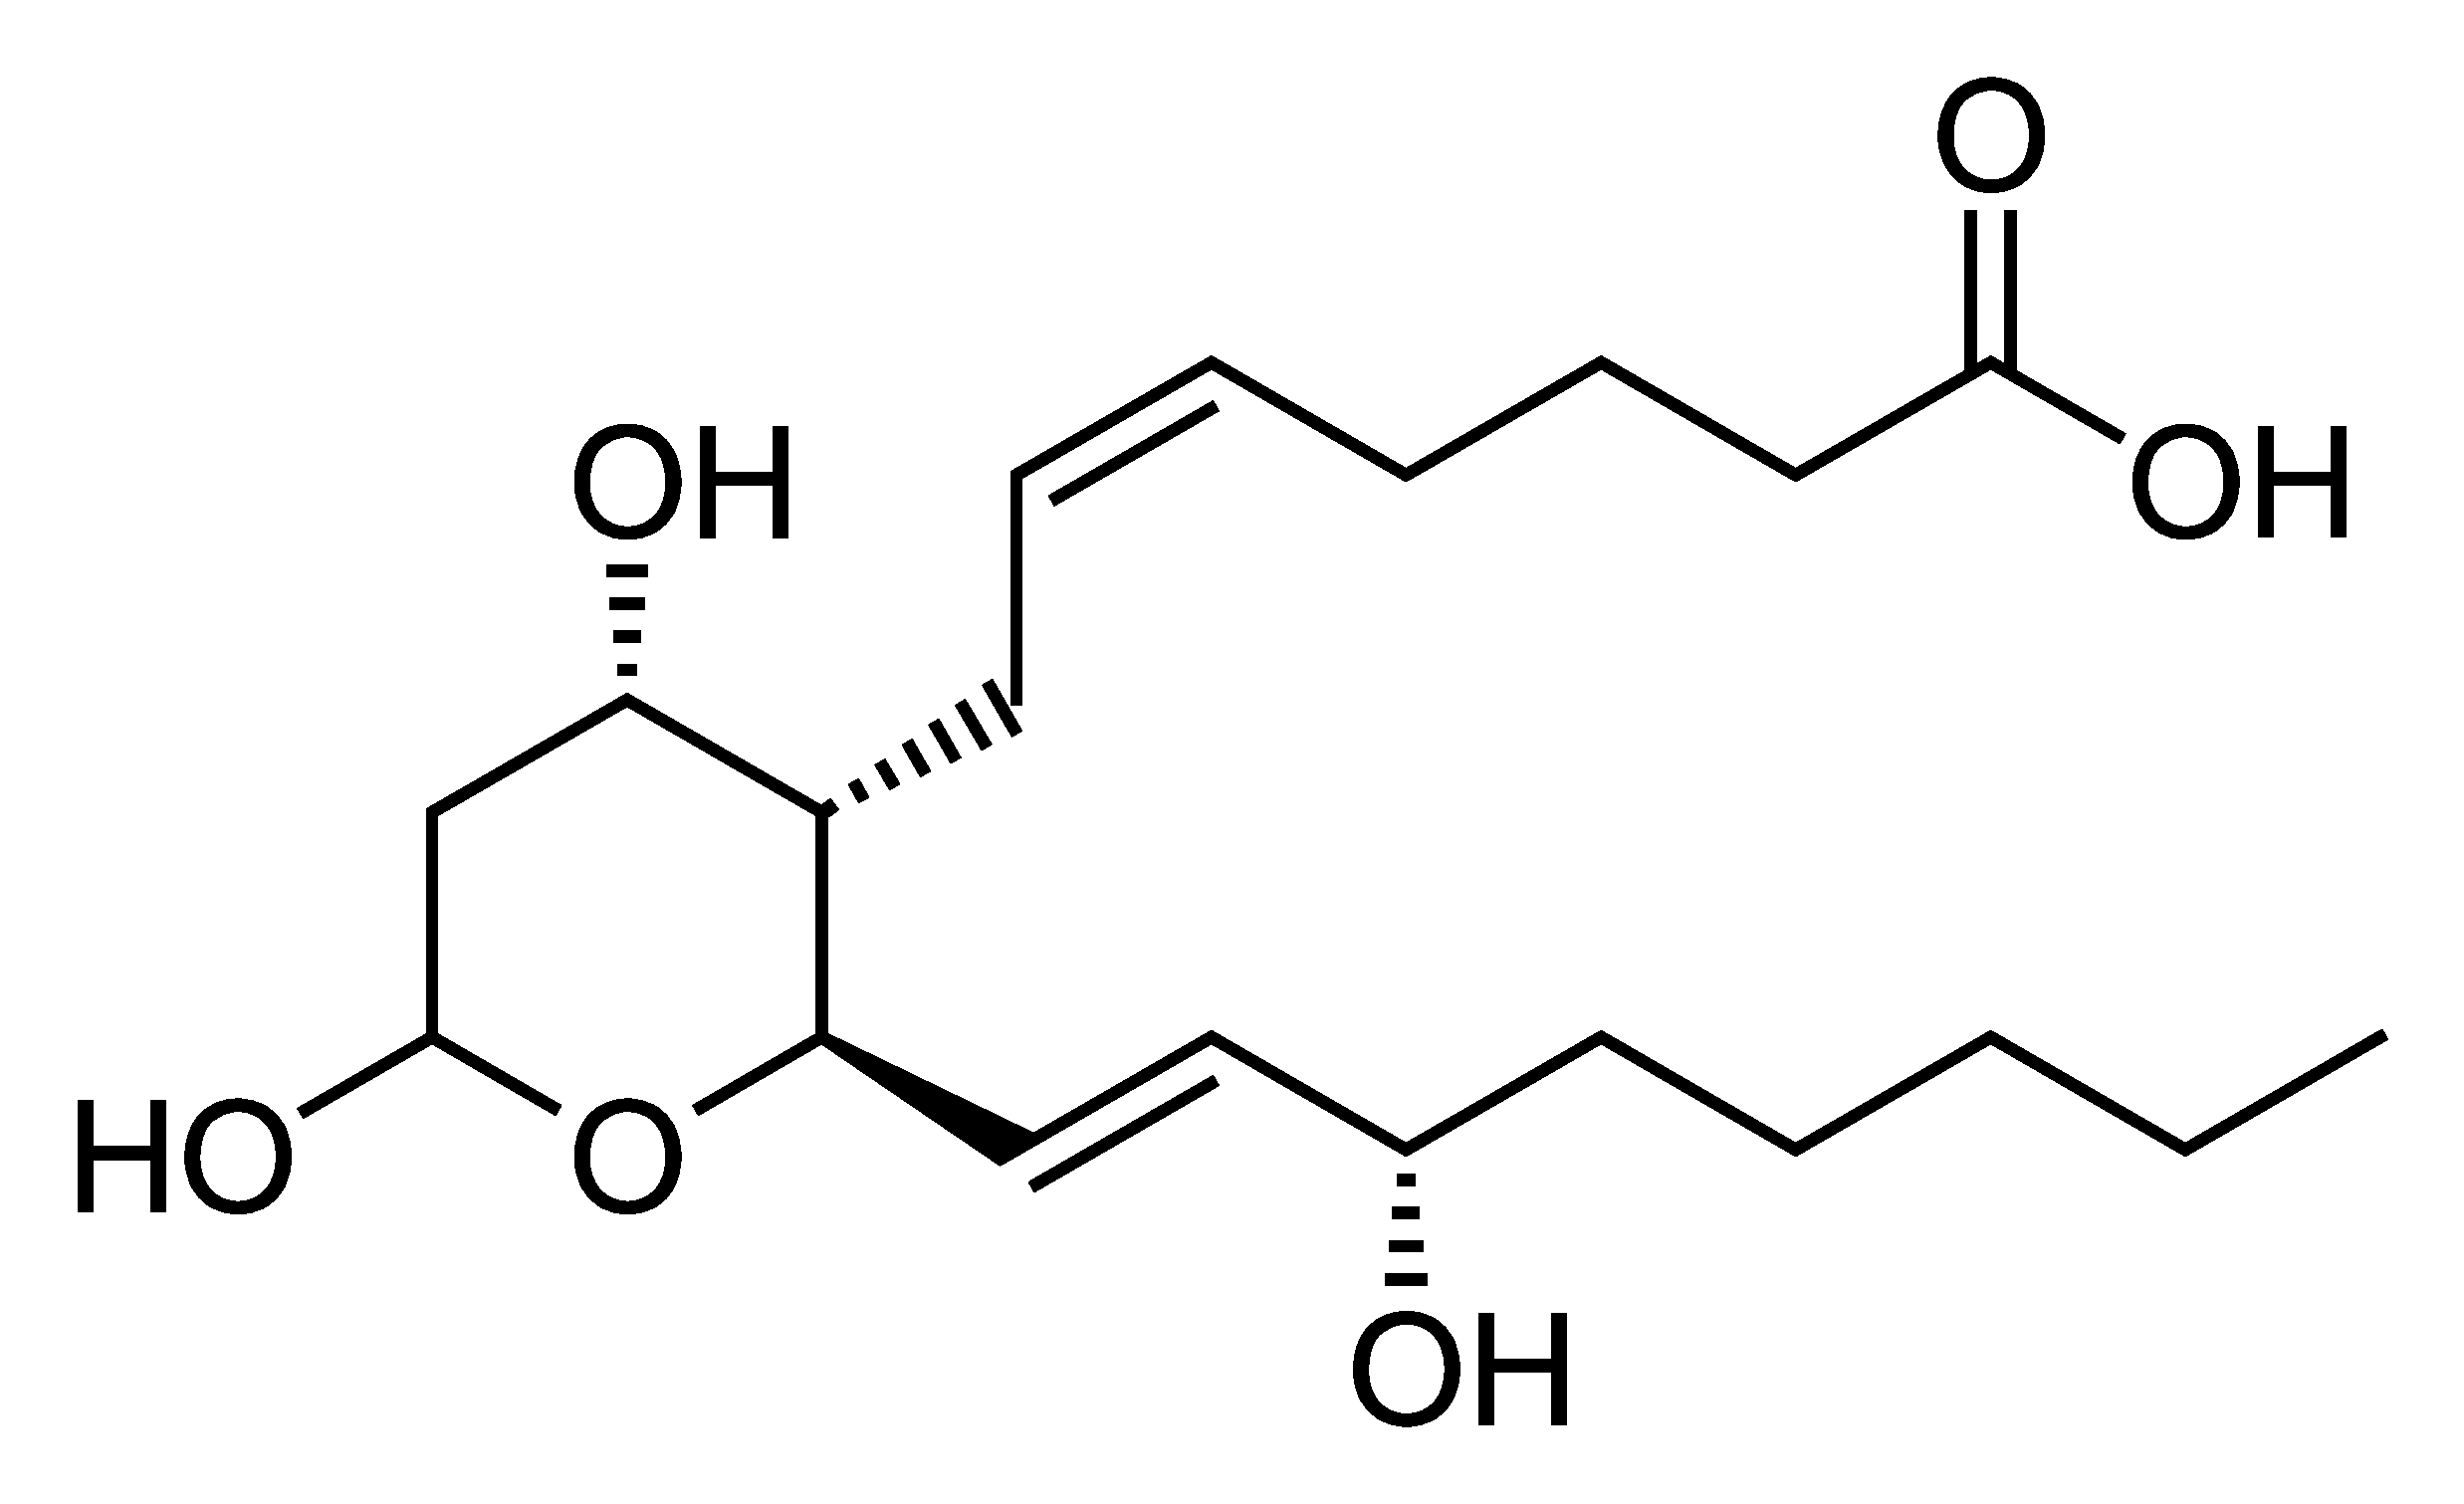
\includegraphics[width=7cm]{Thromboxane_B2.pdf}
    \caption{血栓素 $\mathrm{B_2}$}
\end{figure} 
\footnotetext[5]{Fvasconcellos 16:46, 1 May 2007 (UTC)}

血栓素 (Thromboxane) 又称凝血噁烷,前体也是花生四烯酸。同样具有收缩血管的作用,还会促进血小板凝集。
两种主要的血栓素为血栓素 $\mathrm{A_2}$ 和血栓素 $\mathrm{B_2}$. 

\subsection{非甾体抗炎药对环氧化酶抑制作用}

前列腺素和血栓素的前体均为花生四烯酸,花生四烯酸的前体为细胞膜的重要成分——磷脂。
花生四烯酸在环氧化酶的催化作用下,生成前列腺素和血栓素。

\begin{figure}[htbp]
    \centering
    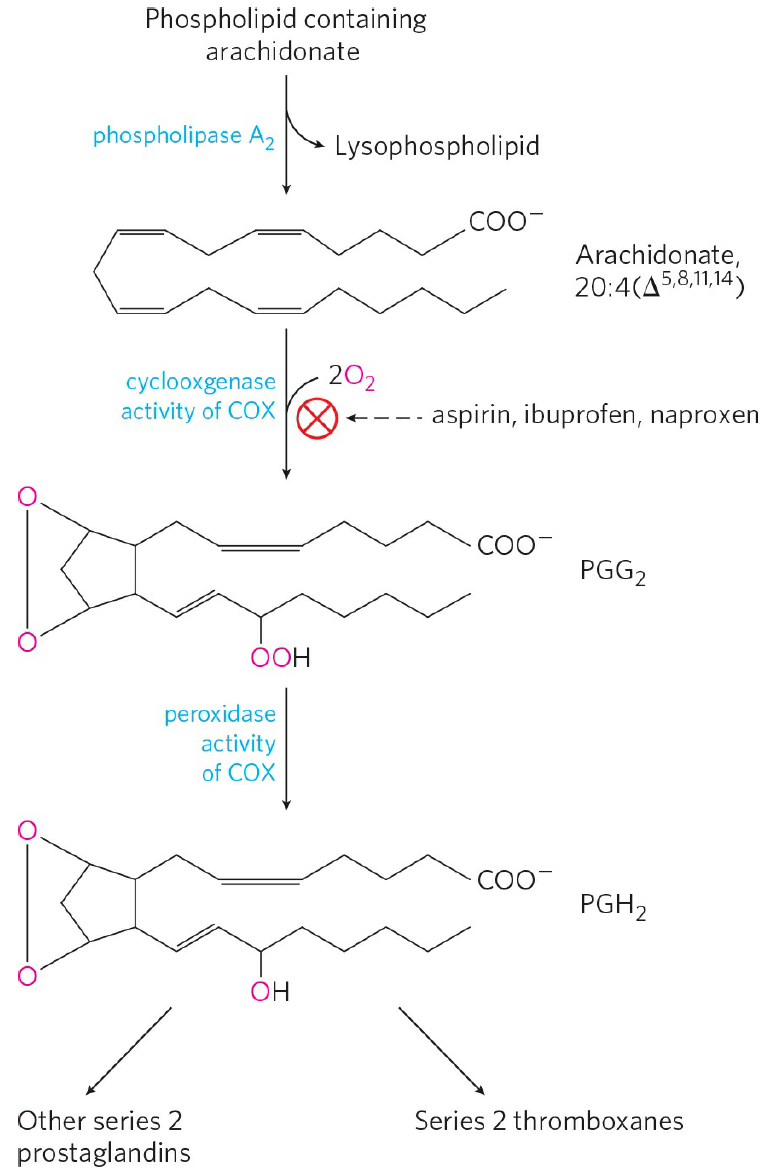
\includegraphics[width=6cm]{Snipaste_2022-11-12_17-55-48.png}
    \caption{前列腺素与血栓素合成过程}
\end{figure} 

环氧化酶在人体内主要有 $\mathrm{COX-1}$ 和 $\mathrm{COX-2}$ 两种。 $\mathrm{COX-1}$ 在胃肠道、肝、肾等器官中均有存在,而
$\mathrm{COX-2}$ 主要存在于炎性环境中。通常,将只抑制 $\mathrm{COX-2}$ 的非甾体抗炎药称为选择性非甾体抗炎药。
相对的,非选择性非甾体抗炎药会同时抑制两种环氧化酶。

非甾体类抗炎药一般抑制环氧化酶活性中心的丝氨酸残基。除阿司匹林外,其他非甾体抗炎药均是可逆性的抑制,阿司匹林
会将丝氨酸残基乙酰化,这个过程是不可逆的。

\newpage
\section{常见非甾体抗炎药}
\subsection{非选择性非甾体抗炎药}
由于非甾体抗炎药作用原理基本相同,所以这里仅介绍使用最广泛、副作用小的布洛芬。

\begin{figure}[htbp]
    \centering
    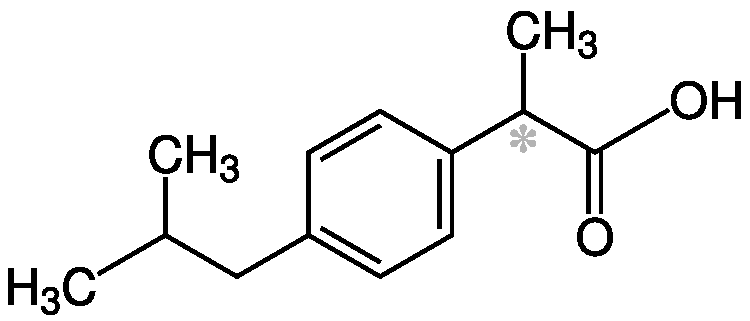
\includegraphics[width=6cm]{RS_-Ibuprofen_Structural_Formula_V1.pdf}
    \caption{布洛芬 RS-Ibuprofen}
\end{figure} 

布洛芬通常用于止疼退热,通常在服用后一小时起效。由于没有选择性地抑制  $\mathrm{COX-1}$ 和 $\mathrm{COX-2}$ 
布洛芬和其他非选择性非甾体抗炎药一样,对胃肠道有刺激作用,但相对其他药的副作用风险较小,可以在饭后服用以降低对胃肠道的损伤。

布洛芬是非处方药,通常被制成缓释胶囊或片剂,药效长达 12 小时。需要注意的是,非甾体抗炎药最适合在疼痛初期使用,
以防前列腺素大量合成,止疼效果减弱。

\begin{figure}[htbp]
    \centering
    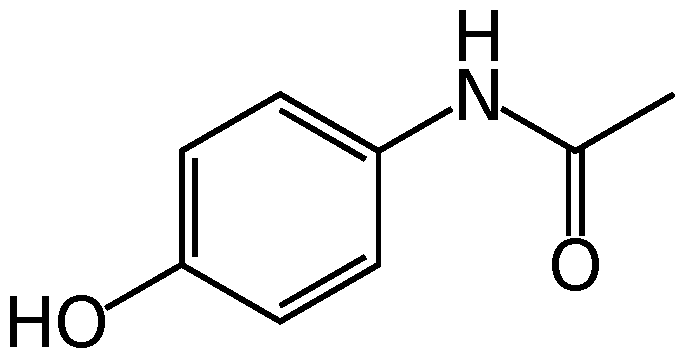
\includegraphics[width=4cm]{Paracetamol-skeletal.pdf}
    \caption{对乙酰氨基酚/扑热息痛 Paracetamol}
\end{figure} 

有一个例外是对乙酰氨基酚(扑热息痛),通常不被认为是非甾体抗炎药,尽管其能抑制环氧化酶。
主要原因是对乙酰氨基酚主要抑制下丘脑中的 $\mathrm{COX-2}$,而对其他部位的环氧化酶抑制作用较弱,
无法起明显的抗炎作用。

\footnotetext[7]{by Denwet}
\footnotetext[8]{by Benjah-bmm27}

\subsection{选择性非甾体抗炎药}

\begin{figure}[htbp]
    \centering
    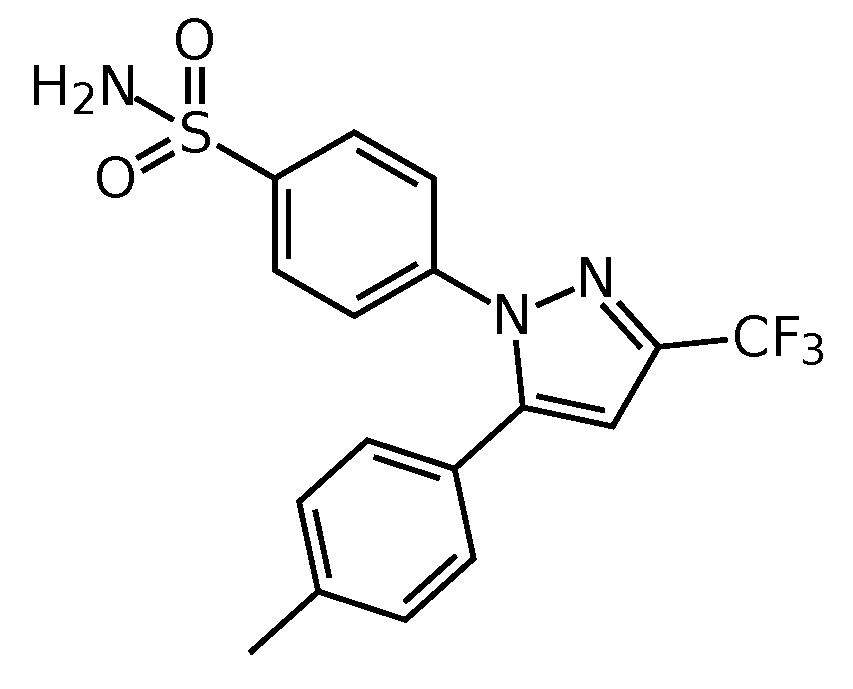
\includegraphics[width=6cm]{Celecoxib.pdf}
    \caption{塞来昔布 Celecoxib}
\end{figure} 
\footnotetext[9]{by Acdx}

塞来昔布是常用的选择性非甾体抗炎药,商品名为希乐葆 (Celebrex),由辉瑞公司研发,目前仍在专利有效期内。
通常用于治疗骨关节炎或其他急性疼痛。这一类药物只抑制 $\mathrm{COX-2}$,因为 $\mathrm{COX-2}$ 主要存在于炎性环境,
所以在起到消炎镇痛作用的同时,胃肠道及其他器官的 $\mathrm{COX-1}$ 仍能正常发挥作用,所以对胃黏膜的损伤较小。
相对的,这类药物的价格要高得多。

虽然这类药物对胃肠道的刺激性较小,但是也有其他的副作用。例如会提高罹患心血管疾病\cite{ref3}、肾衰竭的风险,可有可能会诱发心脏病
提高血栓和中风的概率。目前只有一些经过改良的选择性非甾体抗炎药如塞来昔布和美洛昔康仍在市。

\newpage
\section{非甾体抗炎药用药注意事项}
\subsection{与咖啡因联用}

\begin{figure}[htbp]
    \centering
    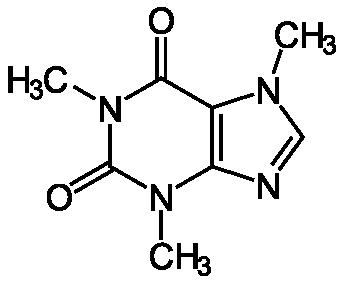
\includegraphics[width=5cm]{Caffeine.pdf}
    \caption{咖啡因 Caffeine}
\end{figure} 
\footnotetext[10]{by NEUROtiker}

咖啡因是一种生物碱,是一种中枢神经兴奋剂,也是腺苷的拮抗剂。

腺苷是一种人体睡眠诱导因子,是 $\mathrm{ATP}$
的代谢产物,在大脑中与腺苷受体结合,会使人产生困意。咖啡因也能与腺苷受体结合,但不会激活腺苷受体,
可以长时间使大脑保持兴奋,并产生更多的肾上腺素,提高心率和血压,并提高身体的新陈代谢效率\cite{ref4}。

在大脑中,有些神经元同时具有腺苷受体和多巴胺受体。咖啡因分子和腺苷分子都是六边形,但是咖啡因分子要略小于腺苷分子。
如果腺苷分子与同时具有腺苷受体和多巴胺受体的神经元结合,会导致多巴胺受体的构象发生改变,无法结合多巴胺分子。
所以适当摄入咖啡因能加大多巴胺的作用效果,是我们更快乐。

多数药物与咖啡因联用能提高药物的作用效果,例如由咖啡因和对乙酰氨基酚制成的酚咖片。
与非甾体抗炎药类似的是,如果以提神为目的摄入咖啡因,最好是在困意产生之前摄入。
因为如果腺苷已经和腺苷受体结合,那么咖啡因就没有机会结合更多的腺苷受体了。
需要注意的咖啡因会促进胃酸的分泌,
虽然能加强非甾体抗炎药的效果,但是同时副作用也会加强,所以最好在饭后服用。
另外,咖啡因还是一种利尿剂,在服用含有咖啡因的药物后,需要注意补水。


\subsection{非甾体抗炎药对胃黏膜的损伤}
非甾体抗炎药的适应症很多,几乎可以说是一种「万能药」,但其副作用同样不能忽视。
前面已经提到非甾体抗炎药会抑制前列腺素对胃黏膜的保护作用,可以通过同时服用胃黏膜保护剂\cite{ref5}来减少其对胃肠道的损伤。
常见的胃黏膜保护剂有铝碳酸镁咀嚼片,在服用后不仅能反应掉一部分胃酸,还能在胃的表面形成一层保护层,促进胃溃疡恢复。

为了减轻非甾体抗炎药对副作用,需要注意合理用药。用于抗炎不宜超过 3 天,用于止痛不宜超过 5 天。
也不能同时服用多种非甾体抗炎药,这样不仅不会加强抗炎效果,反而会使副作用累加。

\newpage
\section{非甾体抗炎药的研发方向}
\subsection{选择性非甾体抗炎药}
非甾体抗炎药新药研制方向之一就是开发 $\mathrm{COX-2}$ 选择性药物,以减轻对胃肠道副作用。
需要注意的是,研发选择性非甾体抗炎药时也要对其进行其他方面的改良,防止产生新的副作用。

\subsection{$\mathrm{NO}$ 释放型非甾体抗炎药}
$\mathrm{NO}$ 调节多种生理功能\cite{ref6},能调节血管张力和血压,在保护胃黏膜的作用上与前列腺素基本相同,
而且与前列腺素有协同作用。所以可以在非甾体抗炎药上引入一个能释放 $\mathrm{NO}$ 的基团,在达到更强的抗炎镇痛作用同时,
降低对胃肠道的不良反应。

\subsection{双重抑制型非甾体抗炎药}
传统非甾体抗炎药只抑制环氧化酶的活性,而花生四烯酸还可以通过 $\mathrm{5-}$脂氧酶 ($\mathrm{5-LOX}$) 产生大量白三烯等炎症因子\cite{ref7}。
因此可以研制同时抑制 $\mathrm{COX}$ 和 $\mathrm{5-LOX}$ 两种酶的抗炎药以达到更全面的抗炎作用。

\newpage
\section*{致谢}
感谢老师的言传身教,并在课程的结尾给我们一个上台展示的机会,锻炼我们表达能力。

感谢我的女友金诗琪,她在我完成这篇论文期间不离不弃的支持,
让我平淡无奇的学习生活变得五彩斑斓。
精神上的支持好过任何一种非甾体抗炎药。希望我们的未来更加美好。

感谢我的电脑和键盘以及 Leslie Lamport 开发的 \LaTeX \ 排版系统,
它们是我完成这篇论文的重要基础。

感谢陪伴我三年的颈椎病,如果不是因为它,
我也不会没有磕绊地说出「对乙酰氨基酚」「塞来昔布」「盐酸乙哌立松」这种复杂的药名,
更不会深入了解非甾体抗炎药的作用机制。

在今天的中国,优质的高等教育仍是一种及其稀缺的资源。
因此,我必须牢记自己的责任与使命。
希望这篇论文不是学术思考的终点。

% 引用
\begin{thebibliography}{99}

    \bibitem{ref1}https://zh.wikipedia.org/wiki/甾体
    \bibitem{ref2}王佰亮. 皮质类固醇性股骨头坏死发病机制与早期干预研究[D]. 中国协和医科大学, 2007.
    \bibitem{ref3}崔旭蕾, 郭向阳, 任洪智. 非甾体抗炎药及其心血管风险[J]. 临床麻醉学杂志, 2007, 23(003):256-257.
    \bibitem{ref4}易超然, 卫中庆. 咖啡因的药理作用和应用[J]. 医学研究生学报, 2005, 18(3):3.
    \bibitem{ref5}胡裕耀, 王章流, 郑华君,等. 铝碳酸镁片在非甾体抗炎药相关性溃疡治疗中的临床价值[J]. 山西医药杂志:下半月, 2012(10):2.
    \bibitem{ref6}李宜川, 刘国玲. 一氧化氮与心血管疾病及胃肠道疾病的关系研究进展[J]. 中国社区医师(医学专业半月刊), 2008.
    \bibitem{ref7}[1]黄凯, 蒋世云, 陈柳军. 5-脂氧合酶及其抑制剂[J]. 中国生物化学与分子生物学报, 2014.
    
\end{thebibliography}


\end{document}